\section{Our Approach}
\label{sec:approach}

We use Hidden Markov Model(HMM) to model the mind drifting process,
based on our belief that each step of the association is only affected by
the previous step, and that each step of association happens under
certain context. Correspondingly, each state in the HMM model is the
probability distribution of every possible contexts.
And under each certain state, the observable result will be the
relatedness of term B to term A, that is, the probability of thinking of
concept B at the mention of concept A under certain state.

\subsection{Context Transition Matrix}
In HMM model, we can compute the next state from current state,
using the transition matrix of all the possible states. So is it in this case.
Since each state here is the probability distribution of all possible contexts,
we can compute their distribution in the next step if we have
the transition matrix of all contexts. To get the context transition matrix,
we use the link structure information from the three online encyclopedia.
We regard the hyperlink in one page as the drifting from one context
to another. Since we already clustered each page into a context,
if page $a_1$ is under context $C_1$, and page $a_2$ under $C_2$,
then we count the hyperlink to page $a_2$ in page $a_1$ as
a time of transition from context $C_1$ to $C_2$.
So after scanning the whole data source, we can get the number of transition links
between any two concepts. If we have $n$  contexts in total,
we can get an $n\times n$ transition matrix $M$,
and $M_{i,j}$ is the probability to transit to context $j$ from context $i$.
Here is how we compute $M_{i,j}$:
\begin{equation}
M_{i,j}=\frac{link(C_i\rightarrow C_j)}{\sum_{k=1}^nlink(C_i\rightarrow C_k)}
\end{equation}
Here $link(C_i\rightarrow C_j)$ is the number of links from context $C_i$ to $C_j$.
Since each state is the probability distribution of all the contexts, that is,
an $1\times n$ matrix, We can get the next state(also a $1\times n$ matrix) by multiplying
the transition matrix $M$. This is how we do state transition.
\begin{equation}
S_{i+1}=S_i\times M
\end{equation}

\subsection{Relatedness under Context}
When we reach a certain state in HMM model, we can get the corresponding observable
result. Here the observable result is the relatedness between each two terms.
When we know the distribution of the contexts, if we have the relatedness score
under each context, we can compute the observable output.
We define the relatedness from concept $a$ to concept $b$ as the
probability of thinking of concept $b$ at the mention of $a$, thus
it is a one-way score, and it is a direct basic score between each pairs,
different from our final score in the model.

When we compute the basic relatedness score, as we mentioned above,
we have two types of information: the TB co-occurrence, representing
the vertical connection, and the SL co-occurrence, representing
the horizontal connection. Since people will either associate vertically or
horizontally, if we know the probability of the two ways, namely the ratio
$\alpha$ of thinking vertically to horizontally, we can compute the basic
relatedness score using the two types of co-occurrence information, as
\begin{equation}
p(a\rightarrow b|C)=\frac{SL(a,b|C)+\alpha *TB(a\rightarrow b|C)}{\sum_{i=1}^nSL(a,t_i|C)+\alpha *\sum_{j=1}^nTB(a\rightarrow t_j|C)}
\end{equation}
Here $p(a\rightarrow b|C)$ means the relatedness score, namely the probability
from concept $a$ to $b$ under context $C$, and $SL(a,b|C)$ means the
SL co-occurrence of $a$ and $b$ under context $C$,
$TB(a\rightarrow b|C)$ is the TB co-occurrence from
$a$ to $b$ under context $C$, and $t_i,t_j$ represents the concepts
co-occurred with $a$ in a sentence or appeared in $a$'s page.

To learn the parameter $\alpha$ under each context, we conduct an experiment.
We first use the TB and SL co-occurrences respectively to compute the basic
probability under each context:
\begin{equation}
p_TB(a\rightarrow b|C)=\frac{TB(a\rightarrow b|C}{\sum_{i=1}^nTB(a\rightarrow t_i|C)}
\end{equation}
\begin{equation}
p_SL(a\rightarrow b|C)=\frac{SL(a,b|C)}{\sum_{i=1}^nSL(a,t_i|C)}
\end{equation}
We randomly pick a group of words in each context, and for each word(we call it keyword),
we compute its top $k$ related words using the two basic 
probability scores separately,
then we get two word lists with the same size. Next, for each list, we iteratively
enter the keyword and related word in the list together to the search engine,
and record the number of their co-occurrence in the search engine, and add the number
together for each list. Then we use the ratio of the total number as the ratio of
people thinking vertically to horizontally.
\begin{equation}
\alpha (C)=\frac{\sum_{i=1}^n\sum_{j=1}^kGC(K(i), R_{TB}(i,j))}{\sum_{i=1}^n{\sum_{j=1}^kGC(K(i), R_{SL}(i,j))}}
\end{equation}
Here $\alpha (C)$ is the ratio of people thinking vertically to horizontally under context $C$,
$GC(a,b)$ is the co-occurrence of the two terms returned by Google, $K(i)$ is the $i$th keyword
we pick in the context, and $R_{TB}(i,j)$ is the $j$th related word of $K(i)$ in the list
computed by TB co-occurrence, and $R_{SL}(i,j)$ is that 
by SL co-occurrence.

This way we compute $\alpha$ for each context. And since now we can compute
$p(a\rightarrow b|C)$ for each pair of words, once the state given, we can
calculate the observable result $p(a\rightarrow b)$ in this state:
\begin{equation}
p(a\rightarrow b|state)=\sum_{i=1}^np(C_i)p(a\rightarrow b|C_i)
\end{equation}
Well $p(C_i)$ is the probability for the $i$th context given by the state,
and $p(a\rightarrow b|C_i)$ is the relatedness score from $a$ to $b$ given
context $C_i$ as we discussed above.

With the TB co-occurrences, SL co-occurrences and $\alpha$,
we can construct the concept association network. If there is enough 
TB co-occurrences from one term to another, 
or SL co-occurrence between them, we can add an
arrows from one concept to the other.
For practical reason and the fact that people would not drift through 
weak connection, we filtered those weak connection edges with too 
few co-occurrences or too small prior probability under each context. 
Then the complete concept association network can be constructed.
We can control the size or density of the network by adjusting 
the filtering threshold.

\subsection{HMM Model}
As we already have the context transition matrix to compute 
the state transition, and the basic relatedness under each context 
to compute the relatedness score given
certain state, we can run the complete HMM model, and use FORWARD algorithm 
\cite{} to compute the probability of any possible path. 
The major steps to compute the probability
for path like $a\rightarrow b\rightarrow c\rightarrow d$ is as follows:

\begin{enumerate}
\item Get the initial state before mind drifting from the page
of the starting concept.
\item Transit to state $S_1$ from the initial state for the first hop
\item compute $p(a\rightarrow b)$ given state $S_1$
\item return to step 2 to transit to the next state and compute
the probability for the next hop, until all the hops passed, we
complete the path
\item compute the final probability score of the path
\end{enumerate}

\begin{figure}[th]
\centering
\shrink
\epsfig{file=hmm.eps,width=0.7\columnwidth}
\caption{Illustration of Our HMM Model}
\label{fig:hmm}
\shrink
\end{figure}

In step 1, we get the initial state from the encyclopedia page of the
starting term. For state $S_1$ derives from its previous state, but there is
not a previous state, so we get the initial state information from the term's
encyclopedia page. Since each page has several labels, 
and we clustered all these
labels into several contexts in \secref{sec:data}, 
we can find several contexts the page belongs to from its label information. 
and the probability for each context in the initial state can 
be calculated as:
\begin{equation}
p(C_i)=\frac{N_{label}(C_i)}{\sum_{k=1}^nN_{label}(C_k)}
\end{equation}
where $N_{label}(C_i)$ is the number of starting term's labels that belong to context $C_i$,
while $\sum_{k=1}^nN_{label}(C_k)$ is the total number of its labels.

This way we can get the final probability of the path $a\rightarrow b\rightarrow c\rightarrow d$:
\begin{equation}
p(a\rightarrow b\rightarrow c\rightarrow d)=p(a\rightarrow b|S_1)p(b\rightarrow c|S_2)p(c\rightarrow d|S_3)
\end{equation}
while
\begin{equation}
p(a\rightarrow b|S_1)=\sum_{i=1}^np(C_i)p(a\rightarrow b|C_i)
\end{equation}
And $p(C_i)$, the probability distribution of context $C_i$, namely the
state $S_1$, derives from:
\begin{equation}
S_1=S_{init}\times M
\end{equation}
where $S_{init}$ is the probability distribution of the initial state we discussed above,
and $M$ is the context transition matrix.

\subsection{Shortest Path and Relatedness score}
Now we can compute the probability score for each possible path
in the concept association network. Since there can be a bunch of
paths from concept $a$ to concept $b$, and they might be directly connected,
we choose the shortest path
to represent the relatedness from $a$ to $b$, that is, the path with
the largest probability score, representing the strongest connection.
So define the relatedness score from $a$ to $b$ as the largest probability
score from all the possible paths.
\begin{equation}
R(a\rightarrow b)=\max{p(a\rightarrow \ldots \rightarrow b)}
\end{equation}
Then we can use this to get relatedness score for any two terms, and apply it
into applications like recommendation system.
